% !TEX root = ../SCXMLREF.tex


\subsection{Intrusion Detection System}
\label{sec:secbot}


The simple intrusion detection system is designed using an Application-Specific Integrated Circuit (ASIC) which connects to a buzzer and a sensor over a Serial Peripheral Interface (SPI) bus. The system is controlled via the ASIC on the SPI bus. At power-up, the ASIC sends commands over the SPI bus to initialize the sensor and the buzzer. After waiting for 50 milliseconds the ASIC enters its main routine, which makes the buzzer respond to the sensor. The statechart model of this system is limited to the ASIC and captures the initialization of the peripherals and the 50 ms wait. In the interest of simplicity we elide the details of the main routine.

The ASIC starts by initializing the buzzer. This involve sending a message over the SPI bus, but the details are not captured in the first refinement of the model. Once the message is sent (which will be indicated by some event saying that the SPI system is done), the ASIC moves on to initializing the sensor. After the ASIC moves into a waiting state for 50 ms, and finally moves into the state which represents normal operation.

\begin{figure}[]
  \begin{centering}
  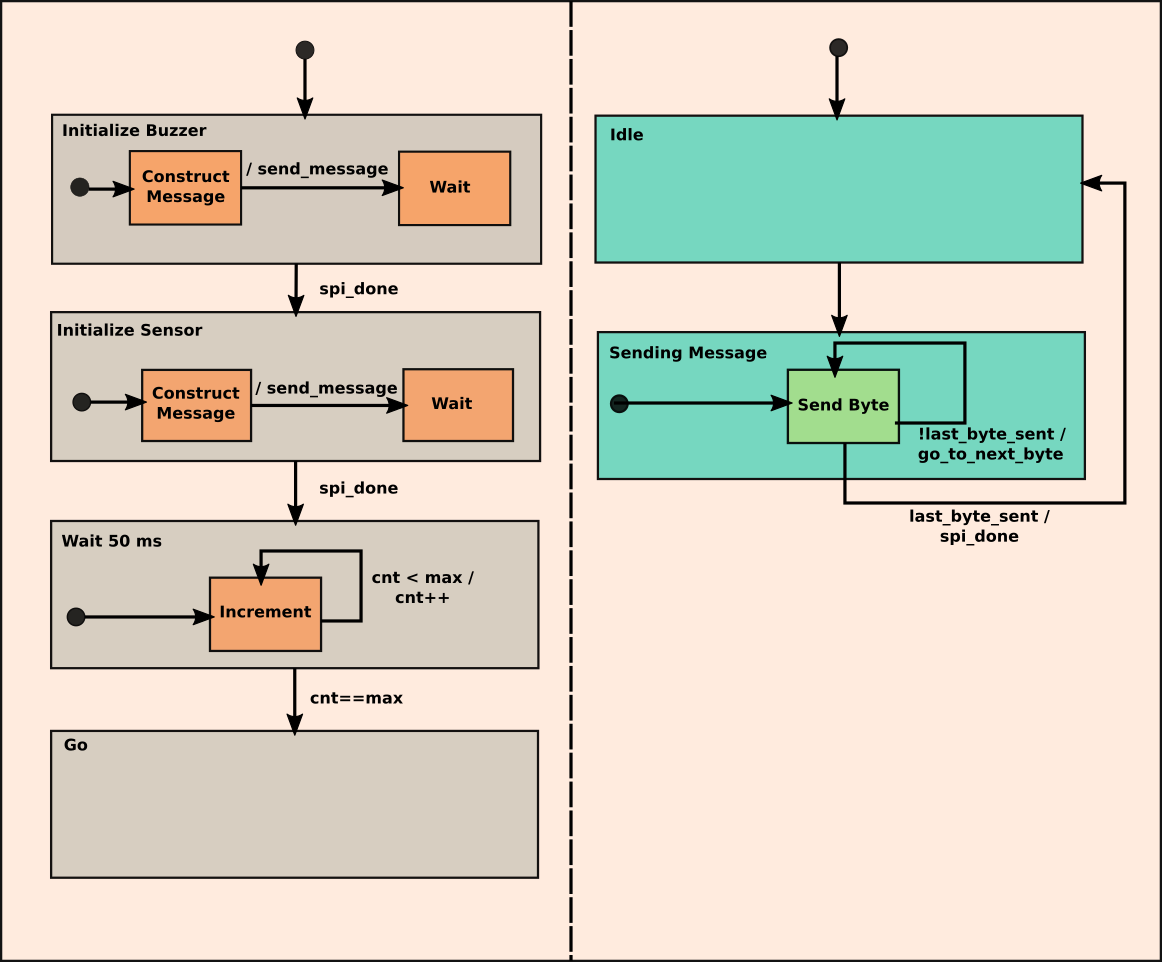
\includegraphics[width=0.6\textwidth]{figures/Buzzer&Sensor_2}
  \caption{Statechart diagram for SecBot intrusion detection system}
  \label{fig:Buzzer}
  \end{centering}
\end{figure} 


\KarlaCommented{Not sure if we should include these figures or the IUMLB generated ones. If we include this figure maybe we can simplify it by using color for each of the refinement levels}
\ColinCommented{introduce the secbot example showing how we would like to develop it in refinements}


